\chapter[Methodology]{Methodology}
\label{Chapter:Methodology}

% Work Objective 
In this work we propose a methodology focused on domain partitioning, that aims to reduce the computational workload and time that would be consumed if we were to train a model on each point of a spatio--temporal domain. We argue that, by considering a number of models generated over representative elements of the domain, which generalize the temporal dimension of other elements, it is possible to preserve a predictive quality comparable to the baseline approach of using a model for every element. As a result of applying the proposed methodology, we could process a spatio--temporal predictive query efficiently while maintaining a low error margin in the prediction.

% Methodology description
The process described by the methodology is divided into two phases, off-line and on-line. The off-line phase comprises three steps: (1) the domain partitioning process, based on clustering partition techniques to find representative elements; (2) the generation of predictive models for the representatives; and (3) a model composition process to predict a subset of the domain region. The on-line phase consists of (4) a mechanism to compute a spatio--temporal predictive query. The methodology is represented by Figure \ref{Fig:OverviewMethodology}: the two main phases are shown in green, the steps for each phase in blue, the tasks performed in every step of the workflow in black and finally the corresponding expected products and outputs are shown in red. 

\begin{figure}[h]
	\centering
	
\includegraphics[scale=0.16]{../Figures/Methodology_Complete}
	\caption{Workflow for the proposed methodology.}
	\label{Fig:OverviewMethodology}
\end{figure}

In Sections \ref{Sec:DomainPartitioning} to \ref{Sec:SpatioTemporalQueryProcessing}, we detail the tasks performed in each step, describing the tools and methods used as well as techniques to validate their performance. The last section discusses the decisions adopted during the development of the methodology.

\section{Step 1: Domain Partitioning}
\label{Sec:DomainPartitioning}

% Objective and general description
The purpose of the domain partitioning is to i) find groups with high similarity according to the temporal evolution on a spatio--temporal domain (in particular univariate time--series) and ii) find representatives for each of the aforementioned groups. We adopt clustering techniques to partition the domain by grouping elements based on a shape similarity measure. In general, a clustering algorithm can be considered as an optimization problem in which we try to minimize the total measure of dissimilarity between the elements in each group \cite{Liao2005}. 

% Consider a representative element
We consider two methods for grouping elements that involve obtaining a representative element (which also exists on the domain) for each group. A representative is then said to generalize the temporal dimension of the other elements in the group. It is important to remember that in a clustering algorithm, the number of clusters, the size of clusters, the definition for outliers, and the definition of the similarity among the univariate time--series are all the concepts which depend on the problem (case study) at hand \cite{Aghabozorgi2015}.

For univariate time--series data, we use the shape--based similarity measure in order to leverage similarities in the temporal behavior of the spatio--temporal domain. In particular, we use Dynamic Time Warping (DTW), previously described in Section \ref{sec:ShapeBasedDistance}.

% What are the products
As part of the off-line process, we calculate the distance matrix that quantifies the DTW similarity between any two time series on the domain. This process can demand considerable computational power, but efficient calculation is possible using data parallelism, by calculating pairwise distances independently and in parallel. Additionally, the distance matrix only needs to be calculated once per domain dataset, and can be saved into persistent storage for future lookups.

In this work we consider the following techniques for the domain partitioning:

\begin{itemize}%[noitemsep,nolistsep]		
	\item $k$--medoids clustering: the purpose of this technique is to group the domain elements that have a high degree of similarity (See Section \ref{Sec:kMedoidsClustering}). As mentioned before, we consider DTW as the similarity measure. 
	
	The benefits of using $k$--medoids as a clustering algorithm are two-fold. In addition to finding the groups that help minimize local dissimilarity, the algorithm returns a medoid for each group, which is an existing object of the domain. For our methodology, we can leverage the model trained on each medoid and measure the generalization error of this model when applied to other points in the corresponding cluster. A downside of $k$--medoids approach is that it requires the computation of the distances between many points, which can have order of time complexity $O(n^2)$. To mitigate this problem, we can leverage a previously calculated distance matrix, which can be reused for all $k$--medoids clusters for that region, thereby significantly reducing the time to compute each $k$--medoids partitioning.
	
	\item Regular or naive partitioning: The spatio--temporal domain is first divided into $k$ rectangles of the same shape (allowing for irregularities when the dimensions cannot be exactly divided) and then, for each given group, we find the element (centroid) that minimizes the total sum of DTW distances to that element. This partitioning is used as a baseline in our methodology to better assess the adequacy of $k$--medoids. This partitioning has no parameters besides the desired number of groups.
\end{itemize}

% Representation of partition profile using the problem formalization
Considering our formal representation in Section \ref{Sec:ProblemFormalization}, we can express the domain partitioning for the spatio--temporal domain $\mathcal{D}$ as follows:

\begin{equation}
\mathcal{D} = \bigcup_{i=1}^{n} \mathbf{S}_{i},
\end{equation}
where for any $i\neq j$ we have that $\mathbf{S}_{i} \cap \mathbf{S}_{j} = \emptyset$, due to the crisp clustering algorithm. And for $\mathbf{S}_{i}$, we admit that a $\mathcal{S}_{i}^{*} \in \mathbf{S}_{i}$ exists (the representative of the group) such that generalizes the temporal dependence of all the elements in $\mathbf{S}_{i}$.

As mentioned in Section \ref{Sec:kMedoidsClustering}, there is the important issue of choosing the number of clusters $k$, which has been recognized as one of the vital issues essential to the success of clustering applications \cite{Aggarwal2013}. Unfortunately, despite the vast amount of expert efforts spent on this matter, there is no consistent and conclusive solution to cluster validation. We will explore some of the available techniques below, on how they are applied to the problem of time series clustering.

\subsection{Determining the number of groups}
\label{Sec:domain_number_groups}

The performance of the $k$--Medoids algorithm is dependent on the optimal value of $k$, the number of clusters to be generated. The $k$--medoids algorithm requires the user to specify the value of $k$, and finding a suitable value automatically is very challenging for time-series data set. The choice is often ambiguous, with interpretations depending on the shape and scale of the distribution of the time--series in a dataset \cite{Liao2005}. An optimal choice of $k$ should strike a balance between maximizing the compression of the data using a single cluster, while maximizing the accuracy when assigning each data point to its own cluster. Here, we explore some of the available methods for finding a suitable value for $k$.

When using a clustering technique for high volumes of data and low variability of the data values throughout neighbor points, it is difficult to determine the optimal number of groups ($k$). This is particularly important for our problem, where there is low variation in the spatial data distribution of the different time-series. 
To identify a cluster in a dataset, we try to minimize the distance between points in a cluster, and the Within-Sum-of-Squares (WSS) method, also know as the Elbow method, measures exactly that. The WSS score is the sum of the squares of the distances of all points within a cluster. Given that the WSS score converges towards zero as the number of groups $k$ goes up to the number of points in the dataset, this method aims to choose a small value of $k$ that still has a low SSE. This is achieved by finding the maximum numerical second derivative for each point, using its two neighboring points (we take into account that the $k$ values are not equidistant when calculating the numerical second derivative). In practice, the elbow represents a point beyond which there are diminishing returns by increasing $k$ \cite{Han2011}.

The average silhouette is another method that assesses the quality of a clustering, by measuring how similar a member is to its own group compared to other groups \cite{Rousseeuw1987}. The silhouette index is a way to measure how close each point in a cluster is to the points in its neighboring clusters. 
Silhouette values lies in the range of $[-1, 1]$. A value close to $+1$ indicates that the sample is far away from its neighboring cluster and very close to the cluster to which it is assigned, meaning it is `well-clustered'. In contrast, a value of $-1$ indicates that the sample is closer to a neighboring cluster than to the cluster to which it is assigned, meaning that it is `misclassified'. A value of $0$ means that it is not clear to which cluster the point should be assigned. 

In this work, we also consider a more refined procedure to find an optimal value for $k$ by means of the inflection point (zero second derivative). But before calculating the second derivative, we apply a cubic smoothing spline to interpolate the values, in order to reduce the noise in the WSS scores. Splines are a smooth and flexible way of fitting Non linear Models and learning the Non linear interactions from the data \cite{HastieTF2009}. This approach should give us another suitable value for $k$.

Comparing partitions approaches, either with each other or with data, is a common requirement in cluster validation. For example, one might hope that different sub-samples of the same data set, or different methods applied to the data, would give similar results. This can also be considered as an aspect of robustness.

% Comparison of the total sum 
In order to assess the robustness of the $k$--medoids clustering algorithm for creating a viable domain partitioning, we compare it against the regular partitioning technique, used as a baseline. Since the $k$--medoids algorithm tries to optimize its cost function (total sum of intra-cluster distances), as opposed to the naive approach of the regular partitioning, we expect that the difference in performance should be more evident as $k$ increases. While larger values of $k$ would tend to lead to clusters with reduced values of the total sum of intra-cluster distances, the techniques for choosing $k$ may not necessarily prefer the largest values of $k$ based on their own cost functions.

In the next Section we describe the methods adopted to built a predictive model for the representative element for every group.

\section{Step 2: Identifying Models for Representatives}
\label{Sec:ModelRepresentatives}

The main objective in this step is to generate predictive models for the representative elements in a domain partitioning. Using these models, we have the ability to compose and/or select those that correspond to a region of interest.

Predictive models can be generated when a forecast method is applied over a time-series in a spatio-temporal domain. In this work, we consider the following forecast methods: Auto-Regressive Integrated Moving Average (ARIMA) and $k$--Nearest Neighbor ($k$NN) models; these two methods are described in Section \ref{Sec:MethodsTSA}. Working with ARIMA model can offer a good trade-off between the predictive accuracy and computational resources to train and predict. The simpler $k$--Nearest Neighbor model is used as a baseline for comparing predictive accuracy.

% Generalization Error and Forecast
In practice, two aspects to forecasting exist: the provision of a forecast for a future value (out-of-sample) of the series and the provision of a forecast error of known values of the series (in-sample). After the process of model tuning, it is possible to test the ability of the model to predict observations that the model didn't see before (as opposed to the fitted values that the model saw throughout the training process). The most common method for evaluating the forecast's success is to predict the actual values with the use of an error metric to quantify the forecast's overall accuracy \cite{Hyndman2006}. The selection of a specific error metric depends on the forecast accuracy's goals. In this work we consider the Root Mean Squared Error (RMSE) and the Symmetric Mean Absolute Percentage Error (sMAPE), both described in Section \ref{Sec:ErrorTSA}.

%following two:

%TODO is this only for in-sample?
% \begin{itemize}
% 	\item Root Mean Squared Error (RMSE): This is the root of the average squared distance of the actual and forecasted values:
% 	\begin{equation}
% 	RMSE = \sqrt{MSE} = \sqrt{\frac{1}{n} \sum_{t=1}^{n} \left(\mathcal{s}_{t} - \mathcal{\hat{s}}_t\right)^{2}}
% 	\end{equation}
% 	Like MSE, the RMSE has a large error rate due to the squared effect and is therefore sensitive to outliers.
% 	\item Mean Absolute Percentage Error (MAPE): This measures the average percentage
% 	absolute error:
% 	\begin{equation}
% 	sMAPE = \frac{200}{n}\sum_{t=1}^{n} \frac{\left|s_t - \hat{s}_t\right|}{\left(s_{t}+\hat{s}_{t}\right)}
% 	\end{equation}	
% \end{itemize}

% Refresh the notation
Recalling the formal representation in Section \ref{Sec:ProblemFormalization}, once we obtain the representative element $\mathcal{S}^{*} \in \mathbf{S}_{i}$, we built $g:\mathbf{S}_{i} \to \mathbf{S}_{i}$ and we can represent $\mathbf{S}_{i}$ using $\mathcal{S}^{*}$ we denote:

%TODO error should have been defined before introducing this equation in formalization
%TODO try to elaborate on the expression of E after explaining forecastings, e.g. f(St - S^t)
\begin{equation}
g^{*}_{i} = \langle \mathcal{S}^{*}, A_p, \mathbf{p}, E, \varSigma \rangle
\end{equation}

%TODO improve this
Thus, the initial approach of having a generic set of models for a domain has been refined, there can now be a reduced number of predictive models that depends on the number of representatives considered. In the case of using a single domain partitioning scheme with $k$ partitions to characterize a domain, there will be $k$ instances of a particular model with $\langle A, p \rangle$ properties. 

As an implementation detail of the off--line process, the predictive models are saved to persistent storage with the appropriate metadata (domain, similarity measure, domain partitioning scheme, group index). This will allow us to recover previously generated predictive models when computing a forecast value for a time-series. The result of applying a partitioning technique to a domain is also stored to speed up future computations.

\section{Step 3: Selecting a Model Representative}
\label{Sec:KnowledgExtraction}

For a given domain partitioning technique and its predictive models for the representatives, we define a ``model composition'' as the subset of representative models that have the ability to compute the prediction/forecast value of the elements in a region of interest on the domain. The model composition computes the RMSE of the forecast error $E_{g^{*}}$ calculated by the models in the intersection $R \cap \bigcup_{i=1}^{k} \mathbf{S}_{i}$ on each element of $R$.  In Figure \ref{Fig:ModelRegion}, we represent the model composition for the region considering the medoid.
\begin{figure}[h]
	\centering
	
\includegraphics[scale=0.35]{../Figures/ModelCompositionRegion}
	\caption{Model Composition using the Representative for a Region $\mathbf{S_{i}}$.}
	\label{Fig:ModelRegion}
\end{figure}

% Solver forecast error analysis
In order to assess the predictive quality of model for the representative element in a given domain partitioning  technique, we compare the generalization error of three other model compositions, in addition to the composition that uses predictive model at the representatives. The four model compositions are described as follows: 

\begin{itemize}%[noitemsep,nolistsep]
	\item Model Composition with Minimal Error: for each group, we find the time series for which its predictive model, when applied to all points of its corresponding group, minimizes the accumulated forecast error. This can be considered the `best' choice for representatives that can only be found through an exhaustive approach.
	\item Model Composition with Minimal Local Error: for each time series $ts_j$ in each group, we train its own model $g_j$ and calculate the corresponding forecast error. We can say that this would be the forecast error of a baseline approach, because it generates as many models as there are time series in the region. This approach should offer the least accumulated forecast error but at a high computational cost, and is the scenario we want to improve on with our methodology.
	\item Model Composition at the Medoids: given the time series of the representatives in each group, we find the corresponding model for each representative, and use it to predict future values of the other time series in their corresponding groups. We then calculate, for each group, the accumulated forecast error when using the model in the representative for all elements in the group. This corresponds to the proposed methodology, and its forecast estimate and generalization error will be evaluated experimentally.
	\item Model Composition with Maximum Error: for each group, we find the time series for which its predictive model, when applied to all poins of its corresponding group, maximizes the accumulated forecast error. This can be considered the `worst' choice for representatives. Together with the Minimal Error, it provides an interval that helps to quantify the appropriateness of the choice of representatives when using the Model Composition at the Medoids.
\end{itemize}

%TODO Describe products
As discussed in the previous Section, in our problem we are not considering a unique $k$ to analyze our methodology, because there is no specific way to optimize the value of $k$. In the following Section we describe the process of building a model composition that is able to leverage several given partitioning schemes.

\subsection{Preparing a Classifier for Representative Models}
\label{Sec:Classifier}

% TODO why: because we need a partitioning scheme, but no way to definitively choose a k, so we use many ks
% TODO desired output of the classifier: given a time series, we want to find the most adequate representative among many different partitioning schemes 

In this section, together with the next, we seek to implement a process that is able to select predictive models using some kind of intelligence, with the aim of finding a composition of models to predict a region of interest with increased accuracy. Here, it is  necessary to remember that, when computing the future value of a variable for a time series, we have to consider a range of values in the immediate past. Thus, in order to create a process for selecting models, we need a mechanism that allows us to find and use relationships between the set of representatives and past temporal instances of every element in the region of interest. 

We formulate this step as a univariate time series multi-class classification problem: Given an unlabeled univariate time series, assign it to one or more predefined classes. For our problem the classes are defined by the identifier of a predictive model on the representative, label composed with the value $k$ and the group index \texttt{cluster\_index} (c.i) where $0 \leq c.i <k$. 

In order to show how we can leverage domain partitioning schemes and their respective representatives, we use the formal representation of the problem (see Section \ref{Sec:ProblemFormalization}), with three different domain partitioning schemes as an example: Given three domain partitioning schemes for a spatio--temporal domain of sizes $m, n$ and $l$ and their respective representative sets, we have:
\begin{eqnarray} 
\nonumber
\mathcal{D}	& = & \bigcup_{i=1}^{m} \mathbf{P_i} \,\,\textrm{and} \,\, \left\{\mathcal{P}_{1}^{m}, \ldots, \mathcal{P}_{m}^{m}\right\},  \\ \nonumber
\mathcal{D} & = & \bigcup_{j=1}^{n} \mathbf{Q_j} \,\,\textrm{and} \,\, \left\{\mathcal{Q}_{1}^{n}, \ldots, \mathcal{Q}_{n}^{n}\right\}, \\ \nonumber 
\mathcal{D} & = & \bigcup_{k=1}^{l} \mathbf{T_k} \,\,\textrm{and} \,\, \left\{\mathcal{T}_{1}^{l}, \ldots, \mathcal{T}_{l}^{l}\right\},
\end{eqnarray}

where $m + n +l < \textrm{card}(\mathcal{D})$. The set of representatives on the partitioning schemes considered is $\mathbf{R} = \left\{\mathcal{P}_{i}^{m}, \ldots, \mathcal{P}_{m}^{m}, \mathcal{Q}_{1}^{n}, \ldots, \mathcal{Q}_{n}^{n}, \mathcal{T}_{1}^{l}, \ldots \mathcal{T}_{l}^{l} \right\}$ , and $\mathcal{G}_{(\mathbf{R})}$ is the set or their correspondent models. Now, for each element in the domain, we want to find some representative $\mathcal{S} \in \mathbf{R}$ that is the representative of some group in a partitioning scheme $\mathbf{P}$, so that the representative satisfies some optimization condition. Here, we choose the representative $\hat{S}$ whose model $g_{\mathcal{\hat{S}}} \in \mathcal{G}_{(\mathbf{R})}$ has the minimum forecast error for the corresponding time series among the other models:

%TODO describir en texto lo que se esta minimizando
\begin{equation}\label{eq:timeseries-representative}
\exists\, \mathcal{\hat{S}} \in \mathbf{R}, \,\, \textrm{such that}, \,\, \argminA_{\substack{\mathcal{\hat{S}} \in \mathbf{R}\\g_{\mathcal{\hat{S}}} \in \mathcal{G}_{(\mathbf{R})}}} E (g_{\mathcal{\hat{S}}}(\mathcal{S})).
\end{equation}

In order to simplify the notation of the aforementioned relationship (\ref{eq:timeseries-representative}), we denote the model with a label \texttt{[number\_of\_clusters, cluster\_index]}, that corresponds to the representative label of the partitioning schemes considered. Assuming that only the number of clusters is used as a parameter for partitioning schemes, this label can uniquely identify each of the representative models, so we can extract a dataset similar to Table \ref{Tab:TSClassificationDataset}.

\begin{table}[h]
	\centering
	%	\tiny
	\begin{tabular}{|c|c|}
		\hline
		Time--Series   & Label for the Representative Model\\ \hline
		$\mathcal{S}_{1}$  & \texttt{[m, 1]} \\ \hline
		$\mathcal{S}_{2}$ & \texttt{[l, l-1]} \\ \hline
		$\mathcal{S}_{3}$ & \texttt{[n, n-2]} \\ \hline
		$\mathcal{S}_{4}$ & \texttt{[l, 2]} \\ \hline
		$\mathcal{S}_{5}$ & \texttt{[m, m-1]} \\ \hline
		$\vdots$       & $\vdots$ \\ \hline
	\end{tabular}
	\caption{Dataset of time-series and labels satisfying relationship (\ref{eq:timeseries-representative}) for domain partitioning sizes $(m,n,l)$.}
	\label{Tab:TSClassificationDataset}
\end{table}

\subsection{Training a Classifier for Representative Models}
\label{Sec:TrainingClassifier}
% Idea of Classifier
For the second part of the model selection process, we are interested in implementing a mechanism based on the knowledge acquired on an extracted dataset (Table \ref{Tab:TSClassificationDataset}). The objective is, given a previously unseen time-series, infer a suitable label (and thus a predictive model on a representative) for it by recognizing patterns in the time-series. This can be formulated as a time--series classification problem, which consists of training a classifier on a dataset $TSD$ in order to map from the space of possible inputs to a probability distribution over the class variable values (labels). 

With the proposed classification method, we will be able to learn from data about the membership relation between elements of the domain and representatives, and then use this learned knowledge to classify new time-series. A dataset $TSD=\{(\mathcal{S}_1,y_1),(\mathcal{S}_2,y_2), \ldots ,(\mathcal{S}_N,y_N)\}$ is a collection of pairs $(\mathcal{S}_i,y_i)$ where $\mathcal{S}_i$ is univariate time series with $y_i$ as its corresponding one-hot label vector of the labels \cite{Gulli2017}. For a dataset containing $m+n+l$ classes, the one-hot label vector $y_i$ is a vector of length $m+n+l$ where each element $j \in [1,(m+n+l)]$ is equal to 1 if the class of $X_i$ is $j$ and $0$ otherwise \cite{Mitsa2010}.

% Multiclass classifier
The task of time-series classification is not a simple one, considering the sequential aspect of time-series data requires the development of algorithms that are able to harness this temporal property select a class label from among a collection of candidates. While many neural network (NN) architectures can be used to solve this problem, some work better than others \cite{Bagnall2017a}. 

In this work we use Convolutional Neural Networks (CNNs), they typically fare very well on multiclass classification tasks, especially for images and text \cite{Goodfellow2016}. The powerful learning ability of deep CNN is primarily due to the use of multiple feature extraction stages that can automatically learn representations from the data. Research has shown that using CNNs for time series classification has several important advantages over other methods; they are highly noise-resistant models, and they are able to extract very informative, deep features, which are independent from time \cite{Wang2016, Bagnall2017a, Zhao2017}.

% https://monkcage.github.io/blog/ai/2019/01/28/time_series_forecast.html
% CNN-LSTM for Time Series Classification
Another architecture are the Long-Short Term Memory Neural Networks (LSTM), the benefit of this model is that the model can support very long input sequences. By implementing an hybrid CNN-LSTM Neural Network, we are able to integrate the capacity of process time-series as blocks or sub-sequences by the CNN model, then pieced together by the LSTM model. Then the model will further divide each sample into further sub-sequences. The CNN model will interpret each sub-sequence and the LSTM will piece together the interpretations form the sub-sequences. 

% TODO picture or example to show how CNN and LSTM work together...

% TODO we got what we wanted, a system that can receive a time series as input, and return a representative model as output.

\section{Step 4: Spatio--Temporal Predictive Query Processing}
\label{Sec:SpatioTemporalQueryProcessing}	

% $R = \langle R, t_p, t_f, Q_{m} \rangle$
In this Section, we describe the on--line process implemented to compute a spatio--temporal predictive query, denoted in Equation \ref{eq:predictivequery}, (see Section \ref{Sec:ProblemFormalization}). The workflow of this process is shown in Figure \ref{Fig:OnLineQP}, and described as follows: 

\begin{figure}[h]
	\centering
	\includegraphics[scale=0.35]{../Figures/Query_Processing}
	\caption{On-Line Processing Spatio-Temporal Predictive Query}
	\label{Fig:OnLineQP}
\end{figure}

\begin{itemize}
    \item [(a)] The input query is processed to extract the query region $R$ and the number of steps $t_p$ (past) and $t_f$ (future).
    \item [(b)] A data validation and extraction from the original dataset are performed according to the input parameters. The data processing for the query consists of the extraction of instances for the query region $R$ joint with past time units $t_{p}$, this means that for each point in $R$ exists a univariate time--series with $t_{p}$ values.
    \item [(c)] When processing a spatio-temporal predictive query, initially we need to determine, for each point in the query region, which predictive models will be used. The model composition is then the resulting set of predictive models used to answer the predictive query with a forecast over the region of interest $R$. Here we implement three types of model composition for analysis:

   \begin{itemize}
	\item Composition of Point Predictive Models: For every point in the region of interest $R$ we use a baseline approach to train a predictive model on each point. This is based on the Model Composition with Minimal Local Error described in Section \ref{Sec:KnowledgExtraction}, but limited to the subset region $R$. To compute the forecast and associated forecast error, we simply use the model on each point.

	\item Composition of Representative Predictive Models: This approach uses the stored information corresponding to the domain partitioning schemes and their respective models. In this type of composition, we require that a domain partitioning scheme (size $k$) is specified as input of the query. Then, we identify the representatives for every point in the query region to load the predictive models that have been previously trained at the representatives. This is based on the Model Composition at the Medoids described in Section \ref{Sec:KnowledgExtraction}, limited to the subset region $R$. For each point in $R$, the model associated to its representative is used to compute the forecast and associated forecast error.
	
	\item Composition of Classifier for Predictive Models: The solver that calculates the result of a prediction query using the outcome of the time-series classifier developed in Section \ref{Sec:TrainingClassifier}. The classifier is a function that, given an input series of size $t_p$, a predetermined suite of partitioning schemes and a region, returns one of the representatives from any of the partitioning schemes that are available in the suite. Once the representative is determined, we follow the procedure for the Model Composition at the Medoids described in Section \ref{Sec:KnowledgExtraction}, but limited to the subset region $R$. This is the main model composition that we wish to evaluate, while the other two are presented for comparisons.
    \end{itemize}
    \item [(d)] With the predictive models obtained from one of the model compositions of the previous step, the requested forecast for the $t_{f}$ steps for each point in $R$ is computed. 
    
    Additionally, if there is information available regarding the actual values of the predictive variable matching the forecast interval, the corresponding error is computed. Otherwise, the generalization error of the model is used. Finally, the errors of the points in $R$ are combined using MSE (see Section \ref{Sec:ErrorTSA}) to produce a single scalar metric for the prediction error over $R$.
\end{itemize}

\section{Summary}
\label{Sec:MethodologySummary}

In this Chapter, we describe tasks and techniques involved in the development for the proposed methodology. Each step uses techniques from different research areas to analyse, explore and extract knowledge from datasets, in particular for univariate time--series.

